%%%%%%%%%%%%%%%%%%%%%
% Likelihood stuff
%%%%%%%%%%%%%%%%%%%%%

% TODO \textcolor{red}{This section has been copied directly from the paper draft. It will be
% expanded upon in a next version.}



The statistical analysis of the observations,  $\{ N^S_i \}$, in the signal region is based on a
likelihood function, $L(\sigma)$, given by
\begin{align}
  L(\sigma) & \equiv  \int   \left[ \prod_{i=1}^M p(N^S_i | \sigma, {\cal L}, \theta_i)  \right] 
\pi(\theta) \, \pi({\cal L}) \, d\theta \, d{\cal L},
\label{eq:marginal}
\end{align}
where $\sigma$ is the total signal cross section, $M = 25$ is the number of bins, $N^S_i$ the
observed count in bin $i$, and the bin-by-bin parameters  $\epsilon$,  $b^S_{QCD}, b^S_{TTJ},
b^S_{\W\ell\nu}$, and $b^S_{oth}$ are  denoted collectively by $\theta$. 
The function $\pi({\cal L})$ is the integrated luminosity prior and $\pi(\theta)$ is an evidence
based prior constructed from observations in the control regions and the four global scale factors
$\kappa^{A/B}_{process}$ determined by simulated data. 
The parameter $\epsilon$ represents the $M$ signal efficiencies (including acceptance) for a given
signal model. Figure~\ref{fig:boost_flowchart} shows which control regions provide constraints on
the background parameters, $b^S_{process}$.
The likelihood per bin is taken to be
\begin{equation}
 p(N^S | \sigma, {\cal L}, \theta) = \textrm{Poisson}(N^S,  \epsilon \sigma {\cal L} + b^S_{QCD} +
b^S_{TTJ} + b^S_{\W\ell\nu} +  b^{S}_{oth}) .
\end{equation}

\begin{figure}[p]
  \centering
  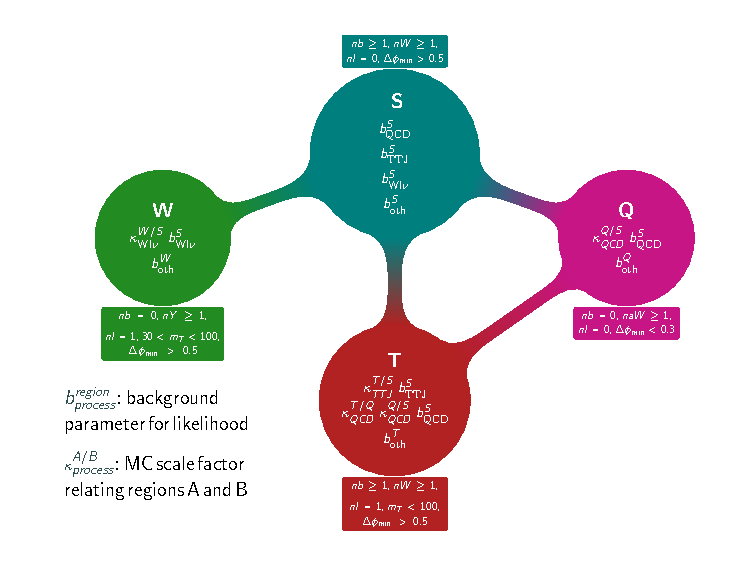
\includegraphics[width=\textwidth]{figures/razor_strategy/BoostFlowChart_noZ}
  \caption{Definition of, and relationship between, the signal ($S$) and control ($Q,T,W$) regions
and their relationship to the bin-by-bin background parameters
$b^{\textrm{region}}_{\textrm{process}}$ for a given region and background process, as well as the
four global scale factors $\kappa^{A/B}_{\textrm{process}} = \sum_i b^A_{\textrm{process}, MC, i} /
\sum_i b^B_{\textrm{process}, MC, i}$, where the sum is over all 25 (\mr,\rsq) bins of the simulated
data. 
The total expected background, per bin, is the sum of the terms shown for each region. Furthermore,
associated with each bin of each region is an observed count $N^{\textrm{region}}$, a simulated
count $N^{\textrm{region}}_{\textrm{process}, MC}$, and a count $N^{\textrm{region}}_{oth, MC}$
equal to the sum of the smaller backgrounds, with associated parameter $b^{\textrm{region}}_{oth}$.
  \label{fig:boost_flowchart}}
\end{figure}

The integral in Eq.~(\ref{eq:marginal}) is approximated by Monte Carlo integration by sampling
 the priors $\pi({\cal L})$, and  $\pi(\theta)$. 
The priors for the expected integrated luminosity, ${\cal L}$, signal efficiencies, $\epsilon$, and 
simulated background counts, $b^{region}_{process, MC}$, are modelled with gamma densities,
\begin{align}
\textrm{gamma}(x, \gamma, \beta) &= \beta^{-1}(x/\beta)^{\gamma-1} \exp(-x / \beta) /
\Gamma(\gamma),
\label{eq:gamma}
\end{align}
in which the mode is set to $c$ and the variance to $\delta c^2$, 
where $c \pm \delta c$ denotes either the measured integrated luminosity, or for a given bin of
a given region and process, the simulated signal efficiency, or the simulated background count. This
yields the gamma density parameters,
\begin{align}
   \gamma &= [(k + 2) + \sqrt{(k+2)^2 - 4}]/2,\\
   \beta &= [\sqrt{c^2 + 4\delta c^2} - c]/2,
\end{align}
where $k = (c / \delta c)^2$.
For empty bins, we set $\gamma = 1$ and the bin value is constrained to zero by setting the $\beta$
parameter to $10^{-4}$.
 
For the signal efficiencies and backgrounds, the prior is modelled hierarchically,
\begin{align}
  \pi(\theta) = \int \pi(\theta | c ) \, \pi(c | \phi ) \pi(\phi) \, dc d\phi,
  \label{eq:prior}
\end{align}
where $c$ is a simulated count or efficiency in an $(\mr,  \rsq)$ bin and $\phi$ represents
parameters that characterize the independent sources of systematic uncertainty, described in
Section~\ref{sec:boost_systematics}. 
The integral in Eq.~(\ref{eq:prior}) is evaluated as follows: $\phi$ values are sampled from
$\pi(\phi)$, then $c$ values from $\pi(c | \phi)$, then $\theta$ values from $\pi(\theta | c)$. 
The sampling from $\pi(\phi)$ and $\pi(\theta|c)$ is straightforward because the functional forms
are known. However, the sampling of $c$ requires running the analysis multiple times.
The independent sources of systematic uncertainty are sampled simultaneously, which produces an
ensemble of sets of $(\mr, \rsq)$ histograms for the simulated backgrounds and efficiencies, for all
signals under consideration, that automatically incorporate all statistical dependencies
without the need to model them explicitly.  The ensemble of histograms is the output of the
procedure described in Section~\ref{sec:boost_systematics}. Thereafter, the sampling proceeds as
follows:
\begin{enumerate}
\item sample the integrated luminosity parameter;
\item sample the efficiency parameters, $\epsilon$, for every signal model;
\item sample the parameters $b^{region}_{process, MC}$ of the simulated background densities and sum
their values over the $M$ bins;
\item compute the $\kappa$ parameters from the appropriate background sums (for example,
$\kappa^{Q/S}_{QCD} =  \sum_i  b^Q_{QCD, MC, i} / \sum b^S_{QCD, MC, i}$);
\item scale each $\kappa$ value by a random Gaussian variate of unit mean and standard deviation
of 0.33 to account for additional uncertainty in $\kappa$ due to deficiencies in the simulated
 data, and 
\item sample the background parameters $b^S_{QCD}$, $b^S_{TTJ}$, and $b^S_{\W\ell\nu}$, from the 
Poisson models  of the control regions; for example, for region $Q$, we map  $\textrm{Poisson}(N^Q
, \kappa^{Q / S} b^S_{QCD} + b^Q_{oth})$ to a posterior density in $b^S_{QCD}$ using a flat prior
and sample $b^S_{QCD}$ from that density.
\end{enumerate}

In the absence of  a signal, we determine limits on the total signal cross section using the CLs
criterion~\cite{LHCCLs} and the test statistic $t_\sigma = 2 \ln [ L(\hat{\sigma}) /  L(\sigma)]$
when $0 \leq\hat{\sigma} \leq \sigma$, and $t_\sigma = 0$ when $\hat{\sigma} > \sigma$. 
Large values of $t_\sigma$ indicate incompatibility between the best fit hypothesis $\sigma^\prime 
= \hat{\sigma}$ and the entertained hypothesis $\sigma^\prime  = \sigma$. 
We calculate  the p-values $p_0 = \textrm{Prob}(t_\sigma > t_{\sigma, obs} | \sigma^\prime = 0)$ 
and $p_\sigma = \textrm{Prob}(t_\sigma > t_{\sigma, obs} | \sigma^\prime=\sigma)$, needed to
calculate $\textrm{CLs}(\sigma) = p_\sigma / p_0$,  by simulation. 
The quantity $t_{\sigma, obs}$ denotes the observed values of the test statistic, one for each
hypothesis $\sigma^\prime=\sigma$.




% \section{Likelihood \label{sec:likelihood}}
% 
% \subsection{Introduction \label{sec:intro}}
% The probability model for this analysis consists of a multi-Poisson 
% likelihood for the signal
% region and a prior that models the uncertainties in 
% the integrated luminosity, ${\cal L}$, the signal efficiencies,
% $\epsilon$ (which includes the
% acceptance), and the backgrounds. The total 
% cross section of the signal,
% $\sigma$, is the parameter of interest. The structure of the model is shown in
% Fig.~\ref{fig:BoostWorkflow}. 
% There is one signal region, $S$, in which the search is conducted and three control regions, $Q$,
% $T$, and  $W$, which are used to constrain the expected QCD, top, and W backgrounds,
% $b^S_{QCD}$, $b^S_{TTJ}$, and $b^S_{W\ell\nu}$, respectively,
%  in the signal region~\footnote{In the symbol
%    $X^{region}_{component}$, the superscript labels the region ---
%    either 
% the signal region, $S$,
%  or a control 
% region, $Q$, $T$, or $W$ --- while the subscript labels the background
% component 
% within the region. Since this analysis uses both real
%  and simulated data, we distinguish symbols pertaining to simulated
%  data  by 
% appending the subscript $MC$.}.
% Simulated data in each of the four
% regions are used to constrain the
% small expected 
% background counts $b_{oth}^j$, $j = S, Q, T, W$ and
% four global scale factors 
% $\kappa^{Q/S}_{QCD}$,  $\kappa^{T/S}_{TTJ}$, $\kappa^{Q/T}_{QCD}$, and
% $\kappa^{W/S}_{QW\ell\nu}$, defined as the ratio of the expected background
% component in a control region to that in the signal (or another control) region.
% For example, the factor $\kappa^{Q/S}_{QCD}$ is the ratio of the
% expected 
% QCD background
% in the $Q$ region to that in the $S$ region. The scale factors can
% be estimated by the inverse of the MC ratios defined in
% Eqs.~(\ref{eq:E1})--(\ref{eq:E4})~\footnote{These
% ratios, which are ratios of
% MC counts, 
% $N^{region}_{component, MC}$ are not used in the model; rather 
% the model is written in terms of the $\kappa$ parameters.}. As noted
% above, global scale factors are used because 
% the statistical precision of some of the
% simulated data precludes the use bin-by-bin scale
% factors. Deficiencies in MC modeling are accounted for by assigning 
% appropriate uncertainties to the global factors, as described in 
% Section~\ref{sec:systematics}.
% 
% 
% 
% Below, we give
% brief 
% descriptions of each of the four 
% regions and provide some details of the statistical modeling. 
% In subscripts, the top contribution is
% written
% as $TTJ$, rather than $TTJ+T$, where it is to be understood that the
% top
% contribution includes single top.
% 
% \subsection{Signal Region}
% 
% Tthe background in the signal region is divided into four components,
% \begin{enumerate}
% 	\item QCD
% 	\item TTJets + T
% 	\item WJets
% 	\item Other (VV, VVV, TTX, Zll, Wbb, Z$\nu\nu$),
% \end{enumerate}
% with expected (i.e., mean) count per bin $b^S_{QCD}$, $b^S_{TTJ}$, $b^S_{Wl\nu}$, and
%  $b^S_{oth}$, respectively. 
% The quantities pertaining to the signal region are:
% \begin{align}
%  \textrm{\bf components}\nonumber\\
%  \textrm{QCD, TTJets+T, WJets, Other}\nonumber\\
%  %
%   \textrm{\bf observed count} 	& \quad\textrm{\bf expected count} \nonumber\\
%   	N^S 
% 	&\quad \sigma \epsilon {\cal L} + b^S_{QCD} + b^S_{TTJ} +
%         b^S_{Wl\nu} +  b^{S}_{oth, MC} 
% 	\nonumber\\
% %
% 	\textrm{\bf MC counts}	& \quad\textrm{\bf expected counts}	
% 	\nonumber\\
% 	N^{S}_{QCD, MC} 		& \quad b^{S}_{QCD, MC}
% 		\nonumber\\ 
% 	N^{S}_{TTJ, MC} 		& \quad b^{S}_{TTJ, MC}  
% 			\nonumber\\ 
% 	N^{S}_{W\ell\nu, MC} 	& \quad b^{S}_{W\ell\nu, MC} 
% 		\nonumber\\ 		
% 	N^{S}_{oth, MC} 		& \quad b^{S}_{oth, MC}	
% \end{align}
% The likelihood per bin is given by, 
% \begin{align}
%   p(N^S| \sigma, \theta) = \textrm{Poisson}(N^S,  \sigma \epsilon {\cal L} + b^S_{QCD} + b^S_{TTJ}
%+ b^S_{Wl\nu} +  b^{S}_{oth, MC}),
%   \label{eq:likelihood}
% \end{align}
% where $\theta$ denotes the nuisance
% parameters $\epsilon$, ${\cal L}$, $b^S_{QCD}, b^S_{TTJ}$,
% $b^S_{Wl\nu}$, and $b^S_{oth, MC}$. 
% The integrated
%  luminosity, the signal efficiency, and the
% simulated background, are modeled 
% with gamma densities, Eq.~(\ref{eq:gamma}).
% 
% 
% \subsection{Control Regions}
% The data counts in a control region are modeled with Poisson distributions, 
% while the
% simulated backgrounds are modeled 
% with gamma densities, Eq.~(\ref{eq:gamma}).
%  
% \paragraph*{Q Region}
% For each bin, this region constrains the parameter $b^S_{QCD}$, given
% $N^Q$, $b^Q_{oth, MC}$ and $\kappa^{Q/S}_{QCD}$.
%  \begin{align}
%  \textrm{\bf components}\nonumber\\
%  \textrm{QCD, Other}\nonumber\\
%  %
%   \textrm{\bf observed count} 	& \quad\textrm{\bf expected count}
%   \nonumber\\
%  	N^Q 					& \quad\kappa^{Q/S}_{QCD} \, b^S_{QCD}  + 
%b^{Q}_{oth, MC} 
% 	\nonumber\\ 
% %
% 	\textrm{\bf MC counts}	& \quad\textrm{\bf expected counts}
% 	\nonumber\\
% 	N^{Q}_{QCD, MC} 		& \quad b^Q_{QCD,MC} = \kappa^{Q/S}_{QCD} \, b^{S}_{QCD, MC}
% 	\nonumber\\ 	
% 	N^{Q}_{oth, MC} 		&\quad b^{Q}_{oth, MC}	
% \end{align}
% 
% \paragraph*{T Region}
% For each bin, this region constrains the parameter $b^S_{TTJ}$, given
% $N^T$, $b^T_{oth, MC}$, $b^S_{QCD}$,  $\kappa^{T/S}_{TTJ}$,
% $\kappa^{T/Q}_{QCD}$, 
% and $\kappa^{Q/S}_{QCD}$.
%  \begin{align}
%  \textrm{\bf components}\nonumber\\
%  \textrm{TTJets, QCD, Other}\nonumber\\
%  %
%   \textrm{\bf observed count} 	& \quad\textrm{\bf expected count}
%   \nonumber\\
%  	N^T 					& \quad\kappa^{T/S}_{TTJ} \, b^S_{TTJ}  
% 	+ \kappa^{T/Q}_{QCD} \, \kappa^{Q/S}_{QCD} \, b^S_{QCD}  
% 	+  b^{T}_{oth, MC} 
% 	\nonumber\\ 
% %
% 	\textrm{\bf MC counts}	& \quad\textrm{\bf expected counts}
% 	\nonumber\\
% 	N^{T}_{TTJ, MC} 		& \quad b^T_{TTJ, MC} = \kappa^{T/S}_{TTJ} \, b^{S}_{TTJ,
%MC}
% 	\nonumber\\ 
% 	N^{T}_{QCD, MC} 		& \quad b^T_{QCD, MC} = \kappa^{T/Q}_{QCD} \,
%\kappa^{Q/S}_{QCD} \, b^{S}_{QCD,MC}  
% 	\nonumber\\ 	
% 	N^{T}_{oth, MC} 		&\quad b^{T}_{oth, MC}
% \end{align}
% 
% \paragraph*{W Region}
% For each bin, this region constrains the parameter $b^S_{W\ell\nu}$, given
% $N^W$, $b^W_{oth, MC}$ and $\kappa^{W/S}_{W\ell\nu}$.
%  \begin{align}
%  \textrm{\bf components}\nonumber\\
%  \textrm{WJets, Other}\nonumber\\
%  %
%   \textrm{\bf observed count} 	& \quad\textrm{\bf expected count}
%   \nonumber\\
%  	N^W					& \quad\kappa^{W/S}_{W\ell\nu} \, b^S_{W\ell\nu}    
% 	+  b^{W}_{oth, MC} 
% 	 \nonumber\\ 
% %
% 	\textrm{\bf MC counts}	& \quad\textrm{\bf expected counts}\nonumber\\
% 	N^{W}_{W\ell\nu, MC} 	& \quad b^W_{W\ell\nu, MC} = \kappa^{W/S}_{W\ell\nu} \,
%b^{S}_{W\ell\nu, MC}
% 	 \nonumber\\ 
% 	N^{W}_{oth, MC} 		&\quad b^{W}_{oth, MC}
% \end{align}
% 
% \subsection{Priors
% \label{sec:priors}}
% The integrated luminosity, the signal efficiencies, and 
% the simulated background counts --- where $c \pm \delta c$ denotes the
% value in an $(\mathrm{M_R}, \mathrm{R^2})$ bin
% and its
% uncertainty --- are modeled with gamma priors of the form, 
% \begin{align}
% \beta^{-1}(x/\beta)^{\gamma-1} \exp(-x / \beta) / \Gamma(\gamma),
% \label{eq:gamma}
% \end{align}
% in which the mode is set to $c$
% and the variance to $\delta c^2$, yielding 
%  \begin{align}
%  	\gamma &= [(k + 2) + \sqrt{(k+2)^2 - 4}]/2,\\
% 	\beta &= [\sqrt{c^2 + 4\delta c^2} - c]/2,
%  \end{align}
% for the gamma density parameters,
%  where $k = (c / \delta c)^2$. For empty bins, $\gamma = 1$ and the bin value is
%  constrained to zero by 
%  setting the $\beta$ parameter to $10^{-4}$.
%  
% \subsection{Final likelihood}
% Several systematic uncertainties in this analysis induce
% correlations
% across the bins of all signal and background models. A canonical example
% is the jet energy scale, which when varied 
% induces coherent shifts in the signal and background
% models. The standard way to
% handle these shifts is to model explicitly (by fitting a large number
% of empirical functions) the
% dependence of the likelihood parameters on the parameters of the underlying sources of
% uncertainty and by making assumptions about how parameters
% are correlated. 
% 
% In this analysis, we  approach the problem
% differently. 
% Uncertainties are accounted for by 
% marginalizing,
% \begin{align}
%   p(D^S| \sigma)	 & = \int   \left[\prod_{i=1}^M p(N^S_i|
%     \sigma, \theta)\right] 
% \pi(\theta) \, d\theta,
% \label{eq:marginal}
% \end{align}
%  the likelihood $p(D^S|\sigma, \theta)$ 
% with respect to an evidence based
% prior $\pi(\theta)$, where $D^S \equiv N^S_1,\cdots, N^S_K$ and $K = 25$
% is
% the number of bins. 
% The integral
% is approximated by Monte Carlo integration,
% \begin{align}
%     p(D^S| \sigma) & \approx \frac{1}{J} \sum_{j=1}^J \prod_{i=1}^K
%     p(N^S_i| \sigma, \theta_j),
% \end{align}
% using $J$ points $\theta_j$ randomly sampled from the prior
% $\pi(\theta)$. Since the
% background model closely matches the data, the points
% $\theta_j$ are well matched to the likelihood. Consequently, 
% with a few hundred 
% points,
% Monte Carlo integration
% provides a good approximation to the integral in Eq.~(\ref{eq:marginal})
% 
% In practice, the prior $\pi(\theta)$ is modeled
% hierarchically,
% \begin{align}
%   \pi(\theta) = \int \pi(\theta | c ) \, \pi(c |
%   \phi ) \pi(\phi) \, dc d\phi,
%   \label{eq:prior}
% \end{align}
% where, again, $c$ is an $(\mathrm{M_R},  \mathrm{R^2})$ bin value 
% and $\phi$ represents parameters that characterize the independent
% sources
% of systematic uncertainty. The integral in Eq.~(\ref{eq:prior}) is
% evaluated
% as follows: one samples $\phi$
% values from
% $\pi(\phi)$,
% then $c$ values from $\pi(c | \phi)$, then $\theta$ values from
% $\pi(\theta | c)$. The sampling from $\pi(\phi)$ and $\pi(\theta|c)$
% is straightforward because the functional forms are known. However, 
% the sampling of $c$ requires running the analysis multiple times.
% 
% 
% One crucial difference with respect to the standard method
% is that we 
% sample \emph{simultaneously} from the priors of the
% independent sources of uncertainty (see
% Section~\ref{sec:systematics}). 
% This procedure produces an
% ensemble of sets of $(\mathrm{M_R}, \mathrm{R^2})$ histograms for
% the simulated backgrounds and the efficiencies for all signals
% under
% consideration. Thereafter, the sampling proceeds as follows. 
% For a given set of $c \pm \delta c$ values:
% \begin{enumerate}
% \item sample the integrated luminosity parameter;
% \item sample the efficiency parameters for every signal model;
% \item sample the parameters $b^{region}_{component, MC}$ of the
% background densities and sum their values over bins;
% \item compute the $\kappa$ parameters from the appropriate 
% background sums (for example,
% $\kappa^{Q/S}_{QCD}$  is given by the ratio $\sum  b^Q_{QCD, MC} /
% \sum b^S_{QCD,
%   MC}$), and 
% \item sample the 
% background parameters of the signal region, $b^S_{QCD}$, $b^S_{TTJ}$,
% and
% $b^S_{W\ell\nu}$, 
% from the 
% Poisson
% models of the control regions~\footnote{The Poisson is
%   inverted
% using Bayes theorem and a flat prior and the background parameter
% is sampled.}. 
% \end{enumerate}
% This sampling technique automatically accounts for all correlations, across 
% all bins, all backgrounds, and all signal models and automatically
% includes any non-Gaussian effects.
% 
